\documentclass{article}
% Change "article" to "report" to get rid of page number on title page
\usepackage{amsmath,amsfonts,amsthm,amssymb}
\usepackage{fancyhdr}
\usepackage{lastpage}
\usepackage{soul,color}
\usepackage{graphicx,float,wrapfig}
\usepackage{hyperref}
\usepackage[scriptsize]{subfigure}
\usepackage{enumerate}
\usepackage[font=small,labelfont=bf]{caption}
\usepackage{listings}
\usepackage{textcomp}
\definecolor{listinggray}{gray}{0.9}
\definecolor{lbcolor}{rgb}{0.9,0.9,0.9}
\lstset{
  tabsize=4,
  rulecolor=,
  language=c++,
  basicstyle=\setstretch{1},
  upquote=true,
  aboveskip={\baselineskip},
  columns=fixed,
  showstringspaces=false,
  extendedchars=true,
  breaklines=true,
  prebreak = \raisebox{0ex}[0ex][0ex]{\ensuremath{\hookleftarrow}},
  showtabs=false,
  showspaces=false,
  showstringspaces=false,
  identifierstyle=\ttfamily,
  keywordstyle=\color[rgb]{0,0,1},
  commentstyle=\color[rgb]{0.133,0.545,0.133},
  stringstyle=\color[rgb]{0.627,0.126,0.941},
}
% In case you need to adjust margins:
\topmargin=-0.45in      %
\evensidemargin=-0.5in     %
\oddsidemargin=-.5in      %
\textwidth=7.0in        %
\textheight=9.2in       %
\headsep=0.25in         %

\newcommand{\answer}{\textbf{\\\underline{ANSWER:}\\}}

% Setup the header and footer
%\pagestyle{fancy}                                                       %
\lhead{\hmwkAuthorName}                                                 %
\chead{\hmwkClass\ - \hmwkTitle}  %
\rhead{Page\ \thepage\ of\ \pageref{LastPage}}                          %
\lfoot{\lastxmark}                                                      %
\cfoot{}                                                                %
\rfoot{}                          %
\renewcommand\headrulewidth{0.4pt}                                      %
%\renewcommand\footrulewidth{0.2pt}                                     %

\fontencoding{T1}
\fontfamily{\rmdefault}
\fontseries{m}
\fontshape{it}
\fontsize{12}{15}
\selectfont

\begin{document}
\begin{center}
\textbf{\textup{\LARGE CS 400/600  Homework \#4}} \\
\textsc{Shumin Guo} \\
\small{Due Date: Nov. 12th, 2010, beginning of the class.}
\end{center}

\textbf{Note: The first several questions are from the textbook.}

\begin{enumerate}
\item(10 points): Let G be a simple connected undirected graph (simple
  graph: no self-edges) with n vertices and m edges. Explain why
  $O(log_2(m))$ is $O(log_2(n))$. 
\answer
For a simple connected undirected graph with n vertices, the smallest
number of edges is $m = n - 1$, and the largest number of edges is $m
= \frac{n(n - 1)}{2}$. So we have the following inequation: \\
$n - 1 \leq m \leq \frac{n(n - 1)}{2} \\
\Rightarrow log_2(n-1) \leq log_2(m) \leq log_2(n) + log_2(n-1) - 1\\
\Rightarrow log_2(n-1) \leq log_2(m) \leq log_2(n)+log_2(n-1)-1 \leq
2log_2(n) \\
\Rightarrow O(log_2(n-1)) \leq O(log_2(m)) \leq O(2log_2(n)) \\ 
\Rightarrow O(log_2(n)) \leq O(log_2(m)) \leq O(log_2(n)) \\
\Rightarrow O(log_2(m))=O(log_2(n))$.

\item (10 points): Let G be a graph whose vertices are the integers 1
  through 8, and let the adjacent vertices of each vertex be given by
  Table \ref{tbl:adj}.

\begin{table}[H]
  \begin{center}
    \begin{tabular}{c|l} 
      \hline
      Vertex & adjacent vertices \\
      \hline
      1 & (2,3,4) \\
      2 & (1,3,4) \\
      3 & (1,2,4) \\
      4 & (1,2,3,6) \\
      5 & (6,7,8) \\
      6 & (4,5,7) \\
      7 & (5,6,8) \\
      8 & (5,7) \\
      \hline
    \end{tabular}
    \caption{Graph adjacent vertices\label{tbl:adj}} 
    \vspace{-15pt}
  \end{center}
\end{table}

Assume that, in a traversal of G, the adjacent vertices of a given
vertex are returned in the same order as they are listed in the above
table.

\begin{enumerate}[a.]
\item Draw G. (See Figure \ref{fig:g2}.)
  \begin{figure}[H]
    \vspace{-20pt}
    \begin{center}
      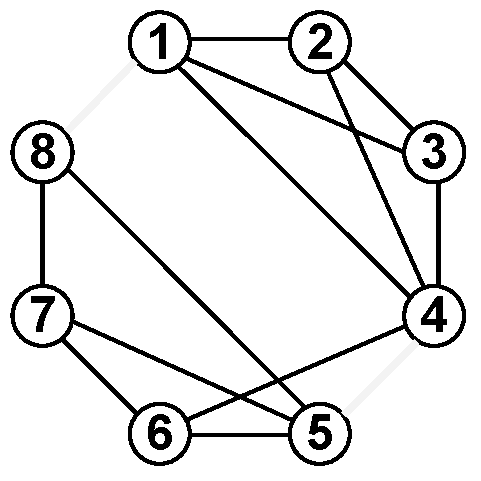
\includegraphics[scale=0.6]{q2-1}
      \caption{Graph for G.\label{fig:g2}}
    \end{center}
    \vspace{-20pt}
  \end{figure}
  
\item Given the sequence of vertices of G visited using a DFS traversal
starting at vertex 1. \fbox{1,2,3,4,6,5,7,8}

\item Give the sequence of vertices visited using a BFS traversal starting
at vertex 1. \fbox{1,2,3,4,6,5,7,8}
\end{enumerate}

\item (10 points): Would you use the adjacency list structure or the
  adjacent matrix structure in each of the following cases? Justify
  your choice. 
\begin{enumerate}[a.]
\item The graph has 10,000 vertices and 20,000 edges, and it is important
to use as little space as possible.
\answer As $n^2=10000^2=10^8\gg 20,000$, there will be a large
percentage of space wasted for storage 0. So in this case, adjacency
list structure is a better choice.
 
\item The graph has 10,000 vertices and 20,000,000 edges, and it is
important to use as little space as possible.
\answer As $n^2=10000^2=10^8$, which is of the same order as
$20,000,000$. But if we store graph using adjacency matrix, still
 $80\%$ of the matrix element is 0. This reason together with the
space constraint requirement make the adjacency list a preferable
choice over adjacency matrix.

\item You need to answer the query areAdjacent() as fast as possible, no
matter how much space you use.
\answer The time complexity of \textbf{areAdjacentVertices()}
operation for adjacency list $O$(min(deg(u),deg(v))) as compared
with $O(1)$ for adjacency matrix makes adjacency matrix the better
choice.

\end{enumerate}

\item (10 points). Given the following directed, weighted graph, show
  the values of the estimated distance matrix, D, at each step of
  Dijkstra$^{\prime}$s algorithm as it searches for the minimal-weight
  path from A to all other vertices, \fbox{See result at Table
    \ref{tbl:dij_alg}}. 
 
\begin{figure}[H]
  \begin{center}
    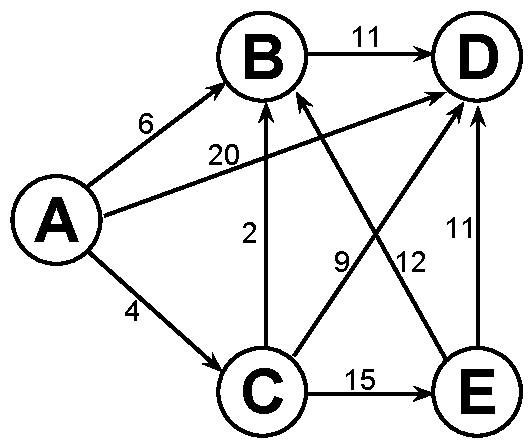
\includegraphics[scale=0.5]{q4-graph}
    \caption{Directed Weighted Graph For Question 4.\label{tbl:dij_alg}}
  \end{center}
  \vspace{-20pt}
\end{figure}

\begin{table}[H]
  \begin{center}
    \begin{tabular}{|c|c|c|c|c|c|} 
      \hline & A & B & C & D & E \\
      \hline Initial & 0 &$\infty$&$\infty$&$\infty$&$\infty$ \\
      \hline A&0&6&4&20&$\infty$ \\
      \hline B&0&6&4&17&$\infty$ \\
      \hline C&0&6&4&13&19 \\
      \hline D&0&6&4&13&19 \\
      \hline E&0&6&4&13&19 \\
      \hline
    \end{tabular}
    \caption{Steps for Dijkstra$^{\prime}$s algorithm. \label{tbl:dij_alg}} 
    \vspace{-15pt}
  \end{center}
\end{table}

\item (20 points). You are given the following weighted
  graph. (See Figure \ref{fig:weighted_undirected}).\\

\begin{figure}[H]
  \vspace{-10pt}
  \begin{center}
    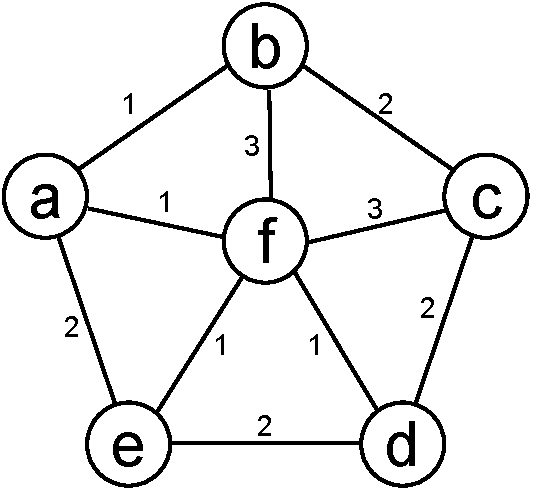
\includegraphics[scale=0.5]{weighted-graph}
    \caption{Weighted Undirected Graph. \label{fig:weighted_undirected}}
  \end{center}
  \vspace{-20pt}
\end{figure}

The adjacency list is: \\
a $->$ b f e\\
b $->$ a c f\\
c $->$ d f b\\
d $->$ f c e\\
e $->$ a f d\\
f $->$ e d c b a

Please use {\it Prim's} and {\it Kruskal's} algorithms, respectively,
to find the minimum spanning tree, and draw the MST at each step. For
the Prim's algorithm, you can assume start with the vertex a. 

Please see Figure \ref{fig:prim} for Prim's Algorithm and Figure
\ref{fig:krus} for Kruskal's Algorithm.

\begin{figure}[H]
  \vspace{-10pt}
  \begin{center}
    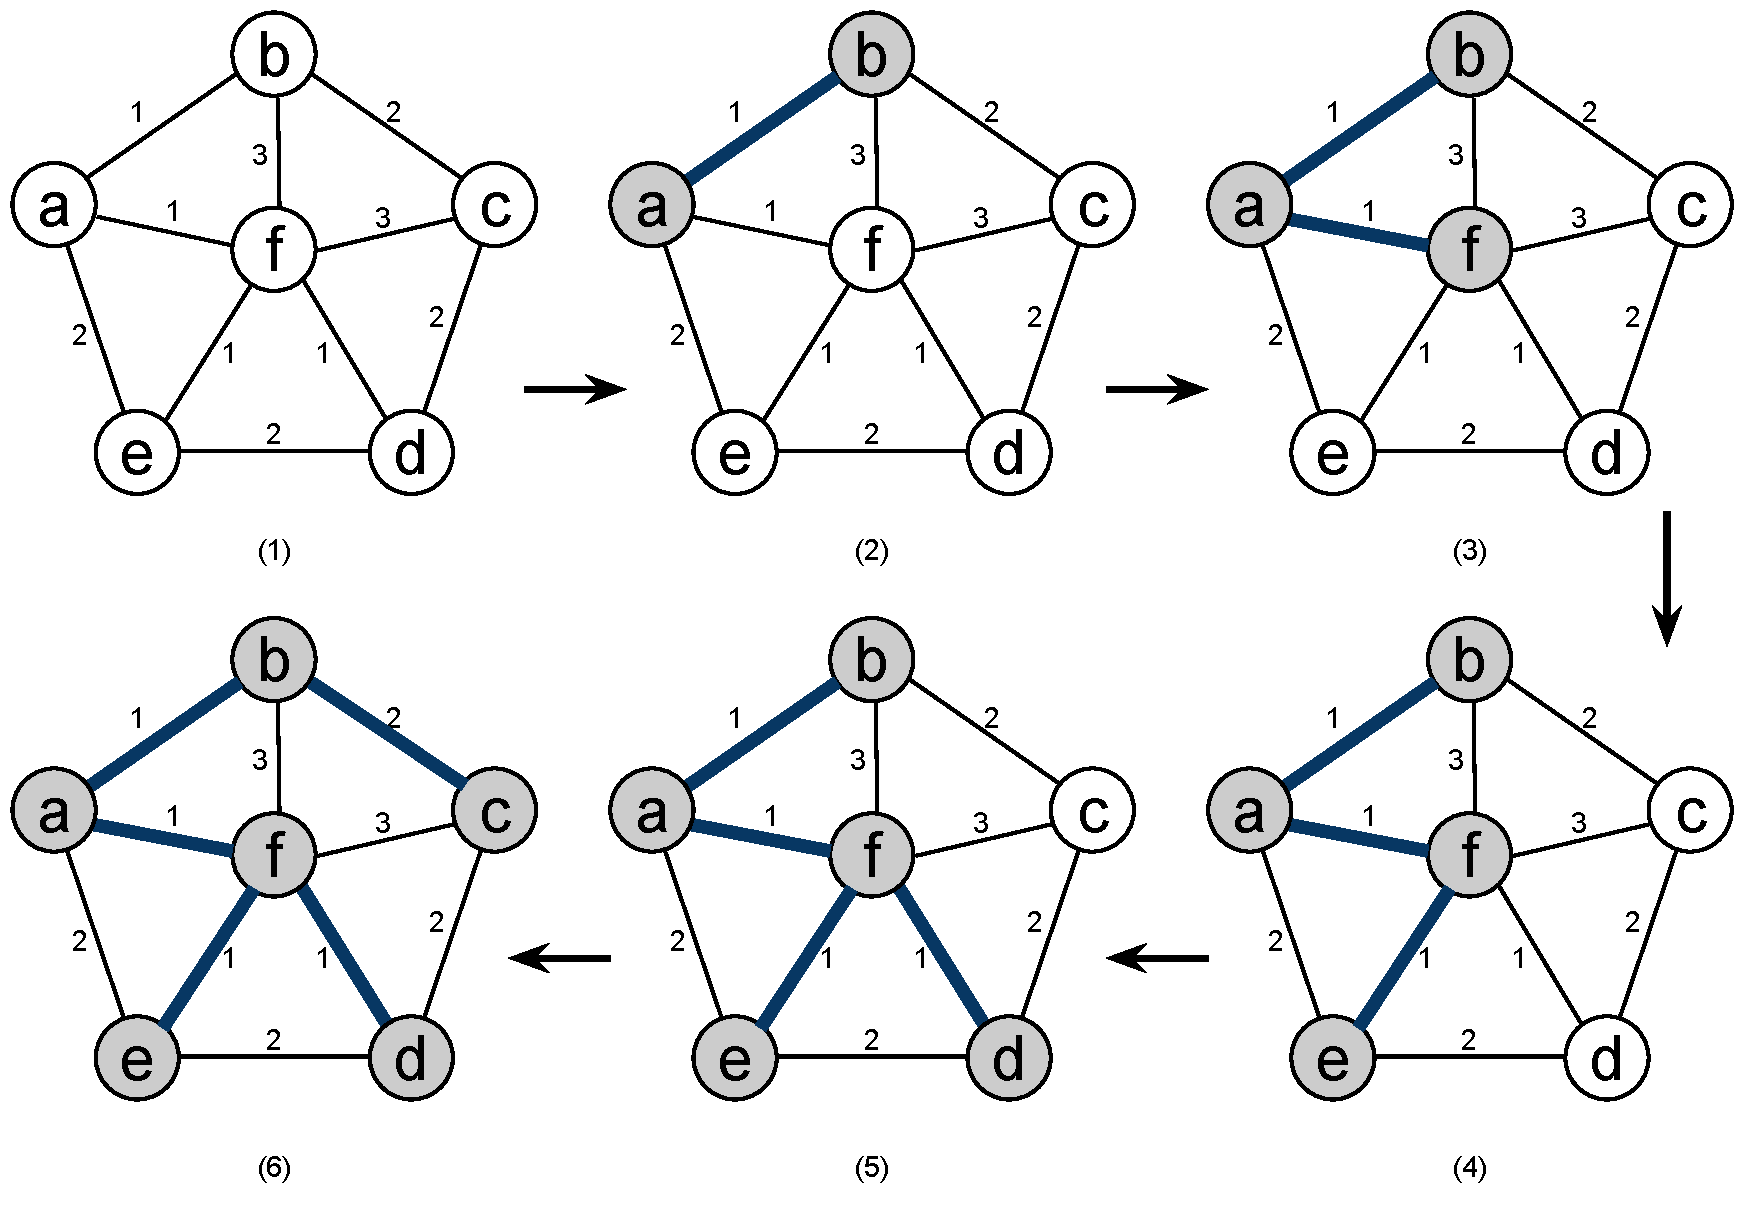
\includegraphics[scale=0.4]{prims_algorithm}
    \caption{Prim's Algorithm Steps.\label{fig:prim}}
  \end{center}
  \vspace{-20pt}
\end{figure}

\begin{figure}[ht]
  \vspace{-10pt}
  \begin{center}
    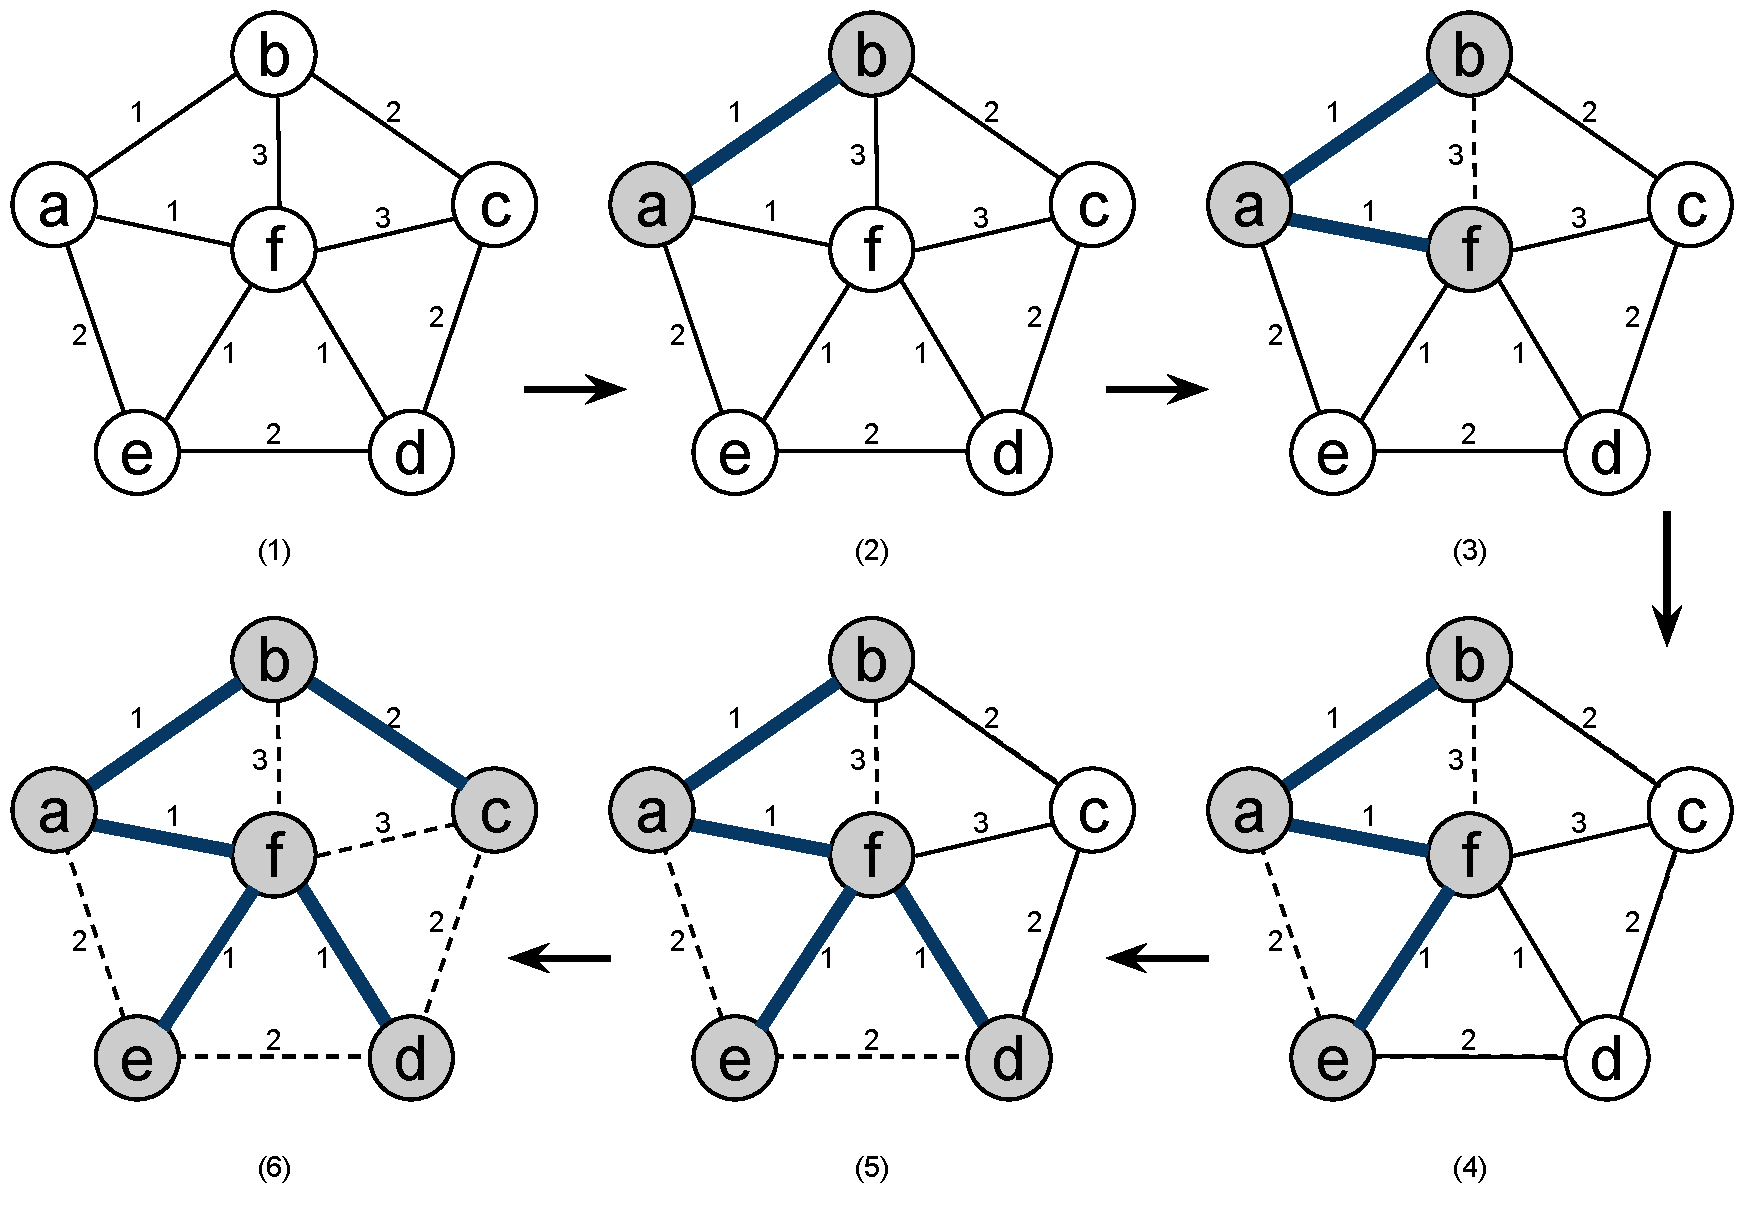
\includegraphics[scale=0.4]{kruskals_algorithm}
    \caption{Kruskal's Algorithm Steps.\label{fig:krus}}
  \end{center}
  \vspace{-20pt}
\end{figure}

\item (15 Points). Do heap sort on the input numbers, 10, 21, 7, 15,
  4, 25. Start by building a min-heap using \textbf{BottomUpHeap()} we
  learned in the class. Give the intermediate result for each step.  
\answer The heapsort begins by building a heap out of the data set,
and then exchange the root(smallest item) with the last item in the
array and remove the last item from the heap. After remove the last
item, it reconstructs the heap and exchange the smallest item with the
last item and do the same thing above. This is repeated until there
is only one item left in the heap. Please see result at Figure
\ref{fig:heap-sort}. 

\begin{figure}[H]
  \vspace{-10pt}
  \begin{center}
    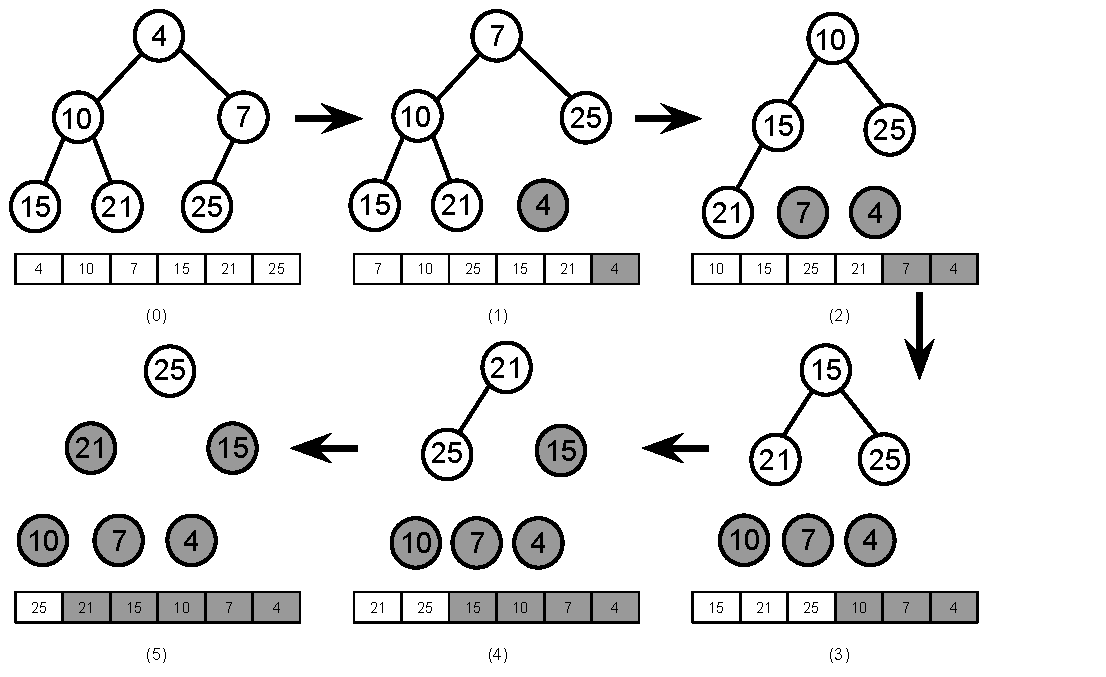
\includegraphics[scale=0.8]{heapsort-steps}
    \caption{Heap Sort Steps.\label{fig:heap-sort}}
  \end{center}
  \vspace{-20pt}
\end{figure}

\item (15 Points). Assume that we always pick the left most element
A[i] in a sequence \textbf{A[i ... j]} as the pivot in the QuickSort
algorithm \textbf{QuickSort(A, i, j)}. Now, assume A is an 8-elements
array, containing a permutation of the number $0, 1, \ldots,7$. Please give
one order of elements in A that QuickSort needs $O(n^2)$ to sort it,
and an example that QuickSort takes $O(nlog_2(n))$.
\answer For quick sort, the best case is when each time we perform a
partition we divide the list into two nearly equal pieces, so that
each recursive call processes a list of half the size. And
consequently, we can make only $log_2(n)$ nested calls before we reach
a list of size 1. This means the height of call tree is $O(log_2(n))$. 
And totally the algorithm uses $O(nlog_2(n))$ time. \\
An example of this case is: \fbox{3,1,0,2,5,4,7,6}

In the worst case, the two sublists have size 0 and n-1 (already
sorted), and the call tree becomes a linear chain of n nested
calls (in this case, the height of quick sort tree becomes n-1). And
the time for the sort will be $T(n)=O(n^2)$.\\ 
An example for this case is: \fbox{0,1,2,3,4,5,6,7}

\item (20 points). Let A[1..n] be an array of n distinct numbers. If $i
  < j $, and $A[i]>A[j]$, then the pair $(i,j)$ is called an inversion of
  A. \\
  a.List all the inversions of the array $< 2, 6, 10, 9, 4>$.
  \fbox{$(2,5),(3,4),(3,5),(4,5)$}. \\
  b.What arrays with elements from the set $\{1,2,\ldots,n\}$ has the
  most inversions? How many does it have? 
  \answer Array $\{n, n-1, \ldots, 2, 1\}$ has the most
  inversions. And the number of inversions is: \\
  \fbox{$n = n-1 + n-2 + \ldots + 2 + 1 = \frac{n(n-1)}{2}$}.

\item (10 points). Which of the algorithms {\it Insertion sort, heap-sort,
  merge-sort}, and {\it quick sort} are stable? Which are in place?
  \answer 
Insertion sort and merge sort are stable\footnote{Quick sort Can be
  implemented as a stable sort depending on how the pivot is handled.}. \\
Insertion sort and heap sort are in place\footnote{Merge sort can be
  implemented as a stable sort based on stable in-place merging}.
\end{enumerate}
\end{document}

%%%%%%%%%%%%%%%%%%%%%%%%%%%%%%%%%%%%%%%%%%%%%%%%%%%%%%%%%%%%%
